\chapter{Ranking of (Semi-)Structured Data}

At its beginning, The Internet was a collection of hypertext documents: textual data with links to additional textual data. At first, search engines were focused on retrieving documents, but with the growth of The Internet, a need for \emph{ranking} documents with regards to how important they are regarding a user's query appeared. Documents consisting only of text, the ranking models assumed as much and no structural information was considered. Nonetheless, some structural cues could still be extracted from the documents, e.g., title, paragraphs, links, \ldots, thanks to the HTML markup are written in. Including these cues into the ranking model improved noticeably its performance.

With the coming of the Semantic Web, documents are turning into a real blend of structured and unstructured data. The structural information is clearly defined. Since this marked a shift of how documents are modelled, there was a need for ranking models to adapt. In this chapter, we present some ranking models used over (semi-)structured data, and introduce the ranking model used in this thesis as a basis for Chapter~\ref{chap:tree-ranking}.

\section{Traditional Ranking Models}

\section{Abstract Model}

\section{Formal Model}

%\section{Entity Model}
%\label{chap:entity-ranking:entity-model}
%
%In this section, we define what is an entity, i.e., the unit of information that is queried and retrieved by an IR search engine. The entity model is based on the graph model presented in Section~\ref{sec:gdm:formal-model}.% In this chapter, we use \emph{document} as an equivalent term for \emph{entity}, since a document is the common term for the object that is ranked in an IR search engine.
%
%An entity in a graph data model is defined as a sub-graph in which a node is considered as the \emph{root}. In RDF the root is the URI that represents that entity, e.g., the URI \url{http://dbpedia.org/page/Earth} for referring to the planet Earth. The edges related to that root form then what we call an \emph{entity}.
%
%\begin{definition}[Entity]
%Let $G = \left\langle V, A, l_V \right\rangle$ be a graph. We call an entity rooted in $u \in V$ a sub-graph of $G$ in which the edges and nodes are a related to the root $u$.
%\end{definition}
%
%There exist several ways to define which edges are related to a root node. We can consider the entity as the connected component that emerges from that root. This can be achieved by performing a breadth-first search starting at the root, and adding the traversed edges and nodes to the entity. Also, one may consider a set of unconnected sub-graphs as the entity according to a similarity measure.
%
%In this chapter, we use the approach described in~\cite{delbru:jws:entity}, where an entity is a star graph, i.e., a sub-graph with a node (the root) and its direct neighbouring nodes it links to. The Figure~\ref{fig:rdf-graph} displays how a graph can be split into four entities \emph{me}, \emph{\_:b1}, \emph{\_:b2} and \emph{paper/547}. Each entity forms a sub-graph containing the incoming and outgoing edges of the root node. In order to simplify the extraction process, we only consider the outgoing edges of a root node.

%\subsubsection{Entity Model}
%
%In the remainder of the paper, the unit of information which is retrieved and ranked is an \emph{entity}~\cite{delbru:jws:entity} and is formalised as a list of attribute-value pairs:
%\begin{description}
%  \item[Entity] represents a set of attribute-value pairs and is identified by the entity node label, e.g., \emph{paper/547};
%  \item[Attribute] is an edge linking the entity node to one of its neighbour nodes and is identified by the edge label, e.g., \emph{title}, \emph{name} or \emph{creator};
%  \item[Value] is a neighbour node of the entity node and is identified by the node label, e.g., \emph{Object-} or \emph{paper/547}. A value is always associated to one attribute. Multiple values can be associated to a same attribute, such as the nodes \emph{\_:b1} and \emph{\_:b2} with the attribute \emph{knows} of the entity \emph{me}.
%\end{description}

\begin{figure}
\centering
\resizebox{0.65\textwidth}{!}{
    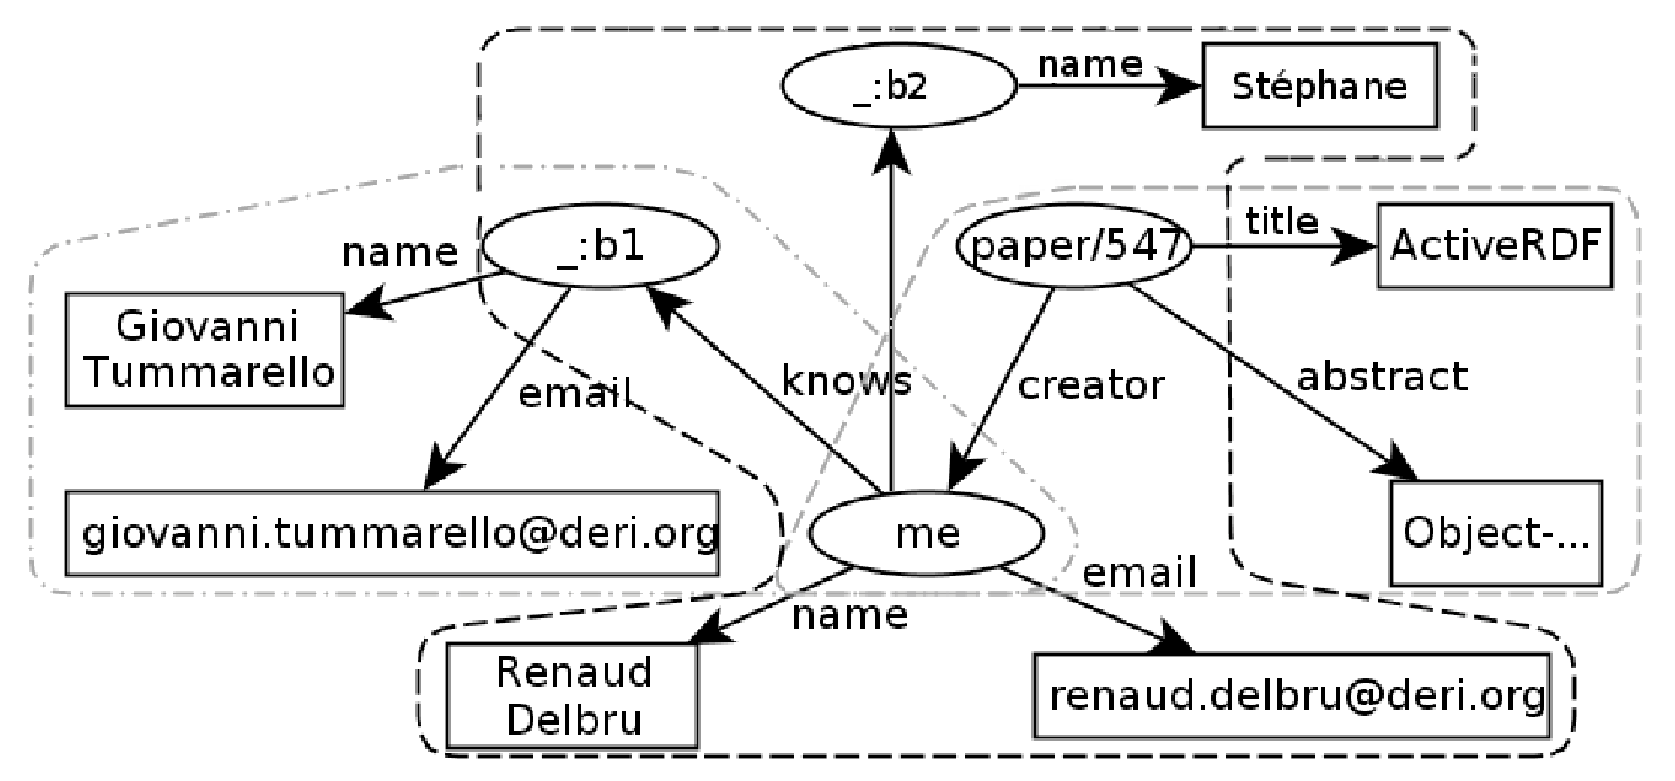
\includegraphics[scale=1]{06-ranking/figures/rdf-graph.eps}
}
\caption{A graph divided into four entities identified by the root nodes \emph{me}, \emph{\_:b1}, \emph{\_:b2} and \emph{paper/547}.}
\label{fig:rdf-graph}
\end{figure}

\subsection{Field-Based Ranking Models}
\label{sec:ranking-wod}

In this section, we explain how to adapt two existing \gls{field}-based ranking frameworks to the entity model.
A field-based ranking model views a document as composed of multiple normalized weighted fields. For example, a field can be the title, the author or the body of the document.

In the Probabilistic Relevance Framework\cite{Robertson:2009:PRF} (PRF), BM25F~\cite{zaragoza:2004:microsoft} is a popular web-search field-based ranking function.
The Divergence From Randomness\cite{amati:2002:acm} (DFR) framework gives birth to many ranking models, in particular to PL2F~\cite{macdonald:2005:clef} which is of the field-based family.

The mapping from the field-based document model to the entity model is straightforward. An entity can be seen as a document and all the edges with a same attribute as a document field. In presence of a multi-valued attribute, the common approach is to merge the content of all the values into one single value, i.e., creating a single bag of words.

\paragraph{Ranking features.}

The following features are used in the field-based ranking functions:
\begin{labeling}{\textbf{average field length}}
	\item[\textbf{field length}] refers to the number of terms in a value node label. In case of a multi-valued attribute, it refers to the number of terms across all the values associated to the attribute.
	\item[\textbf{average field length}] is equal to the mean of \emph{field length} across entities.
\end{labeling}

\paragraph{Normalised term frequency.}

The ranking models presented here are from the \emph{TF-IDF} family, where \emph{TF} is a function of the term frequency, and \emph{IDF} is a function of inverse document frequency. The intuition behind TF is that it captures the relevancy of a term within a document, e.g., the more a term occurs in a document, the more important it is for that document. In contrary, the intuition behind IDF is to capture the importance of a term within the collection of documents: the more a term occur in the collection, the less relevant it is. For example, the term ``food'' would occur frequently in a cooking recipes book, however it may not be an interesting feature in a ranking function.

In general, the term frequency is not used ``as is'' in the TF function, it is first \emph{normalised} before applying the TF function. Term frequency normalisation is useful in cases where the length of a document varies across the collection: it allows to capture this variability into the ranking function, making the score of documents comparable. In \gls{field}-based ranking functions, the term frequency is normalized at the field level, capturing the length variability of a field across documents.

\subsubsection{BM25F Ranking Function}

Using BM25F, an entity $e$ is scored with regard to a query $q$ as follows:
\begin{eqnarray}
Score(e,q) & = & \alpha_e\times\sum_{t\in q}{q_t\times tfn_e \times \omega_t}\\
\label{eq:tfidf-score}
tfn_e & = & \frac{f_{t,e}\times(k_1+1)}{f_{t,e}+k_1} \\
\label{eq:bm25f_2}
f_{t,e} & = &
\sum_{a\in e}{\frac{\alpha_a\times f_{t,e,a}}{1+b_a\times\left(\frac{l_{e,a}}{l_a}-1\right)}}
\label{eq:bm25f_1}
\end{eqnarray}
in which the following notations are used:
\begin{itemize}
	\item $q_t$ is the weight of the query $q$ for the term $t$, i.e., its frequency within the query $q$;
	\item $tfn_e$ is the term frequency normalisation function;
	\item $\omega_t$ is the IDF function of the term $t$;
	\item $k_1$ is the saturation parameter;
	\item $f_{t,e,a}$ is the frequency of the term $t$ in the attribute $a$ of the entity $e$;
	\item $\alpha_a$ is a weight of the attribute $a$ and $\alpha_e$ a weight of the entity $e$;
	\item $b_a$ is the normalisation parameter for the attribute $a$ with $b_a \in \left[0,1\right]$;
	\item $l_{e,a}$ is the \emph{field length} of the attribute $a$ in the entity $e$; and
	\item $l_a$ is the \emph{average field length} of the attribute $a$.
\end{itemize}

The IDF function is defined as
$$
\omega_t=1+log\left(\frac{N}{v_t+1}\right)
$$
where $N$ is the total number of entities in the collection and $v_t$ is the total number of entities that have occurrences of the term $t$.

\subsubsection{PL2F Ranking Function}

DFR ranking models are based on the combination of three components, i.e., the information gain, the randomness model and the term frequency normalisation model. PL2F bases the information gain on the Laplace after-effect model, uses Poisson as the model for randomness, and the \emph{normalisation 2F} for the term frequency normalisation.

Using PL2F, an entity $e$ is scored with regard to a query $q$ as follows:
\begin{eqnarray*}
	Score(e,q) & = & \alpha_e\times\sum_{t\in q}{qtw \times w_{e,t}}\\
	\label{eq:dfr-score}
	w_{e,t} & = & \left(1-P_{risk}\right) \times \left(-log_2\left(P_{P}\right)\right) \\
	\label{eq:dfr-term-weight}
	P_{risk} & = & \frac{tfn_e}{1+tfn} \\
	\label{eq:dfr-prisk}
	P_{P} & = & \frac{\lambda^{tfn_e}}{tfn!}\times e^{-\lambda} \:\text{ where }\: \lambda=\frac{F}{N} \\
	\label{eq:dfr:rand-poisson}
\end{eqnarray*}
in which the following notations are used:
\begin{itemize}
	\item $qtw=\frac{q_t}{q_{t,max}}$ is the weight of the query $q$ for the term $t$ with $q_{t,max}$ the maximum of $q_t$ in $q$;
	\item $w_{e,t}$ is the weight of the term $t$ in the entity $e$;
	\item $1-P_{risk}$ estimates the information gain of a term $t$;
	\item $-log_2\left(P_{P}\right)$ evaluates the importance of a term $t$ in the entity $e$ thanks to the Poisson model; and
	\item $F$ is equal to the frequency of the term $t$ in the collection.
\end{itemize}

The factorial is approximated with the Stirling's formula:
$$
tfn_e!=\sqrt{2\pi}\times tfn^{tfn+0.5}\times e^{-tfn}
$$

The term frequency of the term $t$ in the entity $e$ is normalized as follows:
\begin{equation}
tfn_e = \sum_{a\in e}{\alpha_a\times f_{t,e,a} \times log_2\left(1+c_a\times\frac{l_a}{l_{e,a}}\right)}
\label{eq:pl2f}
\end{equation}
where $c_a$ is a per-attribute hyperparameter with $c_a \in\;]0,+\infty[$.
